\documentclass[aspectratio=43]{beamer}
\usepackage[english]{babel}
\usepackage[utf8]{inputenc}
\usepackage[T1]{fontenc}
\usepackage{textcomp}
\usepackage{appendixnumberbeamer}

\usetheme{unibo}

\usepackage[style=verbose, backend=bibtex]{biblatex}
\bibliography{bibliography.bib}


\AtBeginSection[]{
	\begin{frame}
		\vfill
		\centering
		\begin{beamercolorbox}[sep=8pt,center,shadow=true,rounded=true]{title}
			\usebeamerfont{title}\insertsectionhead\par%
		\end{beamercolorbox}
		\vfill
	\end{frame}
}


\title{Bayesian melding}
\author{Luca Salvatore Lorello (919584)\and Giorgio Tsiotas (934519)}



\begin{document}

\begin{frame}
\titlepage
\end{frame}

\begin{frame}
	\frametitle{Compartmental models}
	\framesubtitle{Introduction}
{\small 	Epidemiological models are a class of models which describe and predict the outcome of infectious diseases. Compartmental models exploit the assumption of a large population by treating the pool of individuals as different compartments which change in size over time.
	
	Many compartmental models are deterministically described by a set of differential equations and can be complicated arbitrarily by designing how compartments behave, for example:}
	\begin{itemize}
		\item compartments can be split by age,
		\item compartments can be split geographically,
		\item rates can be adjusted to consider symptomatic and asymptomatic cases,
		\item natural death causes,
		\item births,
		\item etc.
	\end{itemize}
{\small 	Differential equations can be solved naively with the Euler method:}
\begin{enumerate}
	\item Set each compartment $X \leftarrow X_0$
	\item For $t$ times: $X_{i} \leftarrow X_{i-1} + dX$
	
\end{enumerate}
	
\end{frame}

\begin{frame}
	\frametitle{Compartmental models}
	\framesubtitle{Susceptible-infected-removed (SIR)}
	Only three compartments, governed by the equations:
	\begin{align*}
		dS &= -\frac{\beta S I}{n}\\
		dI &= \frac{\beta S I}{n} - \gamma I\\
		dR &= \gamma I\\
	\end{align*}
	
	This model doesn't take into account reinfections, incubation times or deceased.
	
	\begin{itemize}
		\item $\beta$: infection rate,
		\item $\gamma$: recovery rate,
		\item $n = S + I + R$: total population,
		\item $R_0 = \frac{\beta}{\gamma}$: basic reproduction number,
		\item $R_t = R_0 \frac{S}{n}$: effective reproduction number.
	\end{itemize}
\end{frame}

\begin{frame}
	\frametitle{Compartmental models}
	\framesubtitle{Susceptible-infected-recovered-deceased (SIRD)}
	Four compartments, governed by the equations:
	\begin{align*}
	dS &= -\frac{\beta S I}{n}\\
	dI &= \frac{\beta S I}{n} - \gamma I - f I\\
	dR &= \gamma I\\
	dD &= f I\\
	\end{align*}
	
	{\small This model doesn't take into account reinfections or incubation times.}
	
	\begin{itemize}
		\item $\beta$: infection rate,
		\item $\gamma$: recovery rate,
		\item $f$: fatality rate,
		\item $n = S + I + R$: total population \textbf{still alive},
		\item $R_0 = \frac{\beta}{\gamma}$: basic reproduction number,
		\item $R_t = R_0 \frac{S}{n}$: effective reproduction number.
	\end{itemize}
\end{frame}

\begin{frame}
	\frametitle{Compartmental models}
	\framesubtitle{Susceptible-exposed-infected-recovered-deceased (SEIRD)}
	{\tiny Five compartments, governed by the equations:
	\begin{align*}
	dS &= -\frac{\beta S I}{n}\\
	dE &= \frac{\beta S I}{n} - \sigma E\\
	dI &= \sigma E - \gamma I + c \frac{R I}{n} - f I\\
	dR &= \gamma I - c \frac{R I}{n}\\
	dD &= f I\\
	\end{align*}
	
	This model also takes into account reinfections and incubation times.}
	
	\begin{itemize}
		\item $\beta$: infection rate,
		\item $\sigma$: incubation rate,
		\item $\gamma$: recovery rate,
		\item $c$: reinfection rate,
		\item $f$: fatality rate,
		\item $n = S + E + I + R$: total population \textbf{still alive},
		\item $R_0 = \frac{\beta}{\gamma}$: basic reproduction number,
		\item $R_t = R_0 \frac{S}{n}$: effective reproduction number.
	\end{itemize}
\end{frame}

\begin{frame}
	\frametitle{Compartmental models}
	\framesubtitle{Problems with SEIRD}
	The SEIRD model is very expressive, but it has problems:
	\begin{itemize}
		\item the $E$ compartment is difficult (or impossible) to measure,
		\item the reinfection rate can be hard to estimate (especially in new diseases like COVID-19),
		\item too many degrees of freedom (eg. the $I$ compartment can be tuned by changing 4 different parameters), combined with the uncertainty of measures (eg. is the estimate on the size of $I$ compartment good or there are asymptomatic cases which make this number wrong?).
	\end{itemize}

	Hiding the $E$ compartment (ie. taking $E_0$ as an initial parameter, but not generating $E_t$ as output) can partially mitigate the first problem during fitting.
\end{frame}

\begin{frame}
	\frametitle{The dataset}
	National trend of COVID-19 cases in Italy published by Protezione Civile:
	\begin{itemize}
		\item multivariate time-series with daily values,
		\item contains missing values, but not on the columns we are interested in,
		\item the $S$ compartment cannot be inferred (we assume an initial value of $6 10^7$ individuals at $t_0$ and decrease it depending on the other compartments),
		\item split into \textbf{disjoint windows} for quick exploration of methods (not the best approach, but a good trade-off between speed and accuracy).
	\end{itemize}
	
\end{frame}

\begin{frame}
	\frametitle{Deterministic seeding}
	\framesubtitle{Scipy's \texttt{curve\_fit}}
	Scipy allows to fit an arbitrary function via non-linear least square optimization using the \texttt{curve\_fit} method.
	Since it requires arrays of dependent and independent variables, the compartmental models need to be implemented in order to work vectorially:
	\begin{itemize}
		\item \texttt{\_\_init\_\_} method: sets the model's parameters,
		\item \texttt{eval\_series(t)} method: returns the predictions at times $0..t$,
		\item \texttt{eval\_last(t)} method: returns only the last prediction (at time $t$), used for melding,
		\item \texttt{$f(t, \beta, \gamma, \dots)$} method: wraps \texttt{eval\_last} in order to work with the parameters passed as arrays and sets the parameters at each call, used by \texttt{curve\_fit}.
	\end{itemize}
	
	Fitting is performed on an ensemble of estimators, each optimized to predict a single window given the parameters at the first day. Values are bounded in $[0, \infty)$ for compartments and in $[0, 1]$ for rates. The initial guess for compartments is the value on the first day of the window, while for rates is $0.5$.
\end{frame}

\begin{frame}
	\frametitle{Deterministic seeding}
	\framesubtitle{Results (3-days windows)}
	\begin{columns}
		\column{0.4\textwidth}
		\begin{figure}
			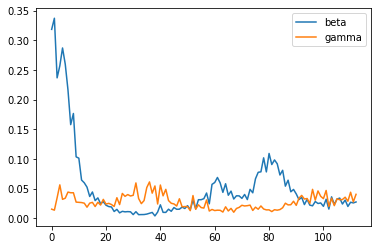
\includegraphics[width=\textwidth]{img/sir_det_3.png}
			\caption{SIR}
		\end{figure}
		\column{0.4\textwidth}
		\begin{figure}
			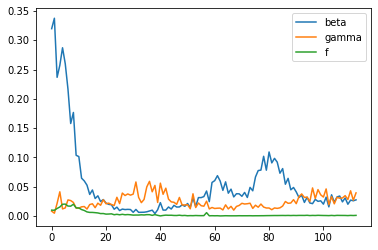
\includegraphics[width=\textwidth]{img/sird_det_3.png}
			\caption{SIRD}
		\end{figure}
		\column{0.4\textwidth}
		\begin{figure}
			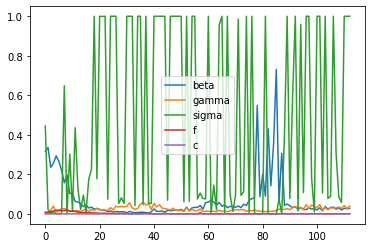
\includegraphics[width=\textwidth]{img/seird_det_1_3.png}
			\caption{SEIRD}
		\end{figure}
	\end{columns}

SEIRD has too many degrees of freedom (also because of hidden $E$ compartment) and in order to fit the observations, the optimizer gives arbitrary values to the parameters (especially $\sigma$).
\end{frame}

\begin{frame}
	\frametitle{Deterministic seeding}
	\framesubtitle{Results (7-days windows)}
	\begin{columns}
				\column{0.4\textwidth}
				\begin{figure}
					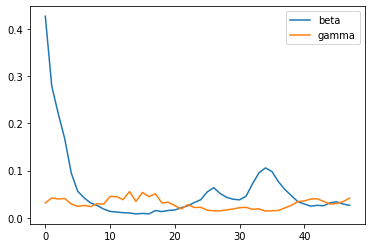
\includegraphics[width=\textwidth]{img/sir_det_7.png}
					\caption{SIR}
				\end{figure}
					\column{0.4\textwidth}
				\begin{figure}
					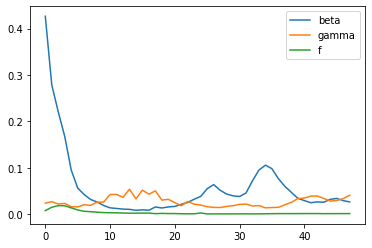
\includegraphics[width=\textwidth]{img/sird_det_7.png}
					\caption{SIRD}
				\end{figure}
				\column{0.4\textwidth}
					\begin{figure}
						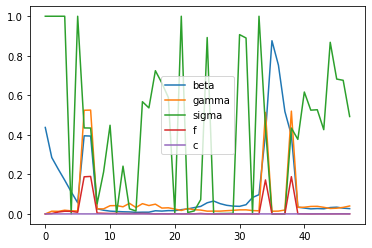
\includegraphics[width=\textwidth]{img/seird_det_1_7.png}
						\caption{SEIRD}
					\end{figure}
	\end{columns}
\end{frame}

\begin{frame}
	\frametitle{Deterministic seeding}
	\framesubtitle{Results (15-days windows)}
	\begin{columns}
		\column{0.4\textwidth}
		\begin{figure}
			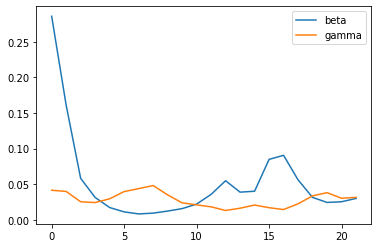
\includegraphics[width=\textwidth]{img/sir_det_15.png}
			\caption{SIR}
		\end{figure}
		\column{0.4\textwidth}
		\begin{figure}
			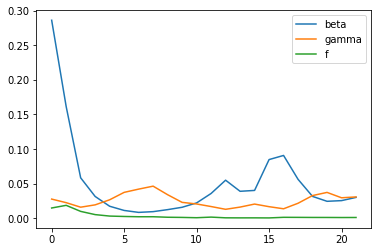
\includegraphics[width=\textwidth]{img/sird_det_15.png}
			\caption{SIRD}
		\end{figure}
		\column{0.4\textwidth}
		\begin{figure}
			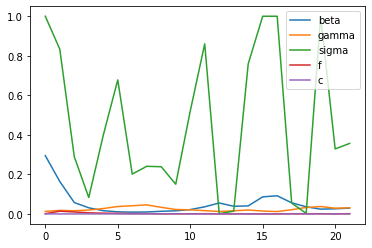
\includegraphics[width=\textwidth]{img/seird_det_1_15.png}
			\caption{SEIRD}
		\end{figure}
	\end{columns}
\end{frame}

\begin{frame}
	\frametitle{Deterministic seeding}
	\framesubtitle{Improving the Hidden SEIRD fit}
	
{\tiny 	In order to constrain the SEIRD model, we bounded $\sigma$ to values from literature~\footfullcite{lauer2020incubation}, but still got spurious spikes. In another test we further narrowed the interval to $0.093 \pm 0.01$ (the average between 8.2 and 15.6 days), obtaining better results.
	
	\begin{columns}
		\column{0.35\textwidth}
		\begin{figure}
			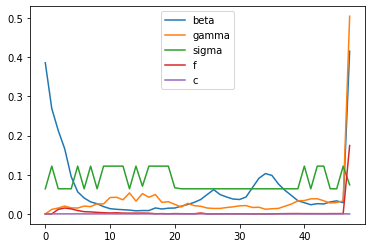
\includegraphics[width=\textwidth]{img/seird_det_2_7.png}
			\caption{SEIRD with $\sigma \in [\frac{1}{15.6}, \frac{1}{8.2}]$ (7-days window)}
		\end{figure}
		\column{0.35\textwidth}
		\begin{figure}
			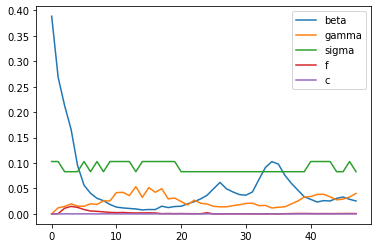
\includegraphics[width=\textwidth]{img/seird_det_3_7.png}
			\caption{SEIRD with $\sigma \in [0.083, 0.103]$ (7-days window)}
		\end{figure}
	\end{columns}
}
\end{frame}


\begin{frame}
	\frametitle{Bayesian melding}
	\framesubtitle{Idea}
{\tiny 	A deterministic model can be seen as a cause-effect relationship between inputs and outputs, however the probabilistic informations available are lost. The most simple approach would be to create a random variable $Y = f(X)$ as the application of the model to the random input, but this would discard all the available informations about the output distribution (ie. the likelihood of each possible outcome).
	
	Bayesian melding is a statistical technique which puts together (meld) all the available informations about inputs and output distributions, without suffering from Borel's paradox (unlike older techniques as Bayesian synthesis).
	\begin{alertblock}{Borel's paradox}
		Conditional probabilities on events with null probability causes the entire pdf not to be reparametrization-invariant (eg. simply changing the scale of variables causes the shape of the pdf to change).
	\end{alertblock}

	\begin{block}{Bayesian melding as consensus among many pdfs}
		A ``coherent'' pdf can be derived by pooling different pdfs. Logarithmic pooling is the only method which preserves \textbf{external Bayesianity} (on multivariate pdfs, applying Bayes theorem before or after creating the joint probability yields the same results).
		\begin{equation*}
		T(q_1, q_2, \dots, q_n) \propto \displaystyle\prod_{i=1}^n q_i^{\alpha_i},\ with\ \displaystyle\sum_{i=1}^n \alpha_i = 1
		\end{equation*}
	\end{block}
}
\end{frame}

\begin{frame}
	\frametitle{Bayesian melding}
	\framesubtitle{Which pdfs to pool?}
	When fitting a deterministic model, we have at our disposal:
	\begin{itemize}
		\item hypotheses on inputs and outputs (priors),
		\item observations from the phenomenon we are trying to model (likelihoods).
	\end{itemize}	
	
	We can meld the output prior $q_2$ and the induced output distribution $q_1^*$ (computed by applying the input prior to the model) to get a ``coherent'' pdf on outputs by a factor $\alpha$, then, applying Bayes theorem, we can condition that pdf to the actual observations:
	\begin{equation*}
		P(\texttt{input} = \theta \mid \texttt{output} = M(\theta)) = (\frac{q_2(M(\theta))}{q_1^*(M(\theta))}) ^ {1-\alpha} L_1(\theta) L_2(M(\theta))
	\end{equation*}
\end{frame}

\begin{frame}
	\frametitle{Bayesian melding}
	\framesubtitle{Sample importance-resampling algorithm}
	In order to compute the induced density, the model needs to be inverted ($q_1^*(M(\Theta)) = q_1(M^{-1}(\Phi))|J(\Theta)|$, where $J$ is the Jacobian of the model in functional form), but this is usually not possible. The sample importance-resampling algorithm allows to bypass this problem, by approximating the pooled distribution as follows:
	\begin{enumerate}
		\item Sample phase: extract a large number of samples from the input prior,
		\item Importance computation phase: weight each sample:
		\begin{enumerate}
			\item run the model on each sample to get the posteriors,
			\item estimate $q_1^*$ from the posteriors with a non-parametric method (eg. Gaussian KDE),
			\item associate each sample $\Theta_i$ to a weight $(\frac{q_2(M(\Theta_i))}{q_1^*(M(\Theta_i))}) ^ {1-\alpha} L_1(\Theta_i) L_2(M(\Theta_i))$,
		\end{enumerate}
	\item Resampling phase: take a small subset of the samples, following the weights computed,
	\item The new samples (approximately) follow the input pdf which best explains the observed outputs (and therefore its mean can be used to fit the model, with the variance as a measure of confidence).
	\end{enumerate}
	
	Execution can be very slow (5 days on SEIRD for the entire dataset split into 7-days windows) due to the large number ($\sim 10^5$) of samples and the posterior estimation.
\end{frame}

\begin{frame}
	\frametitle{Bayesian melding}
	\framesubtitle{Our assumptions on distributions}
	We are dealing with multivariate pdfs, both for inputs and outputs. The joint probability for a given model (eg. SEIRD) can be computed as the product of the marginals, under an independence assumption, or can itself be pooled. We needed to make further assumptions on the probabilities:
	\begin{itemize}
		\item input likelihoods for rates (eg. $\beta$, $\sigma$, etc.) are unknown, therefore they are set as uniform in $[0, 1]$,
		\item input priors for rates were seeded with the results of \texttt{curve\_fit} and set as Gaussians with the given value as mean,
		\item every density related to compartments (both prior and likelihood) set to Gaussians with the known value as mean,
		\item for every marginal density function (except the uniform ones), deciding a variance is very problematic: an initial heuristic for compartments is to take the variance of the values inside the window we want to fit, when this doesn't work, a different value is set.
	\end{itemize}
	
	
	\begin{alertblock}{What happens when no consensus is reached?}
		When the melded pdfs don't have sufficient overlap, underflows and divisions by zero may occur. This makes choosing the right model and priors very important for the outcome.
	\end{alertblock}
\end{frame}

\begin{frame}
	\frametitle{Bayesian melding}
	\framesubtitle{Results (7-days windows, independent marginals assumption)}
	The SEIRD model behaved badly also during least square optimization, therefore its values were averaged (EMA, $\alpha = 0.05$) in order to try to reduce the chance of poor melding.
	
	
	\begin{columns}
		\column{0.4\textwidth}
		\begin{figure}
			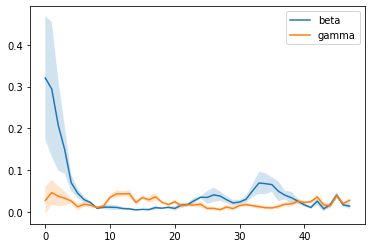
\includegraphics[width=\textwidth]{img/sir_meld_7.png}
			\caption{SIR ($10^4$ samples, $500$ resamples)}
		\end{figure}
		\column{0.4\textwidth}
		\begin{figure}
			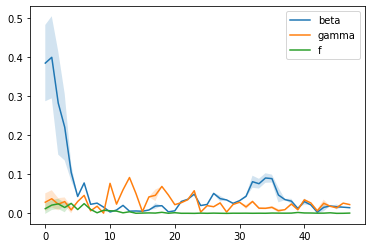
\includegraphics[width=\textwidth]{img/sird_meld_7.png}
			\caption{SIRD ($5 \cdot 10^4$ samples, $2000$ resamples)}
		\end{figure}
		\column{0.4\textwidth}
		\begin{figure}
			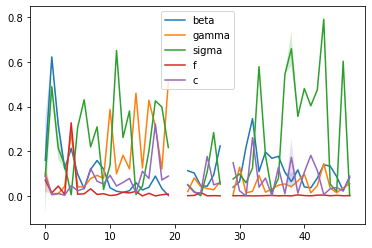
\includegraphics[width=\textwidth]{img/seird_meld_7.png}
			\caption{SEIRD ($10^5$ samples, $5000$ resamples)}
		\end{figure}
	\end{columns}
\end{frame}

\begin{frame}
	\frametitle{Bayesian melding}
	\framesubtitle{Results (7-days windows, marginals pooled geometrically)}
	\begin{columns}
		\column{0.4\textwidth}
		\begin{figure}
			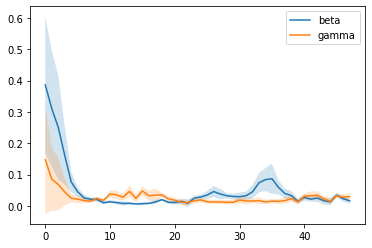
\includegraphics[width=\textwidth]{img/sir_meld_7_log.png}
			\caption{SIR ($10^4$ samples, $500$ resamples)}
		\end{figure}
		\column{0.4\textwidth}
		\begin{figure}
			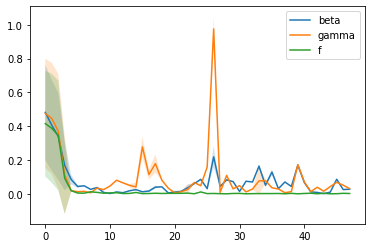
\includegraphics[width=\textwidth]{img/sird_meld_7_log.png}
			\caption{SIRD ($5 \cdot 10^4$ samples, $2000$ resamples)}
		\end{figure}
		\column{0.4\textwidth}
		\begin{figure}
			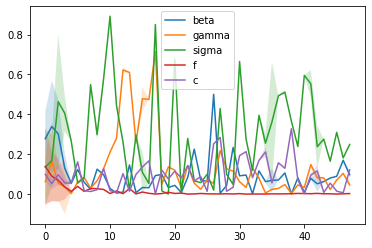
\includegraphics[width=\textwidth]{img/seird_meld_7_log.png}
			\caption{SEIRD ($10^5$ samples, $5000$ resamples)}
		\end{figure}
	\end{columns}
\end{frame}

\begin{frame}
	\frametitle{Bayesian melding}
	\framesubtitle{Results (15-days windows, independent marginals assumption)}
	\begin{columns}
		\column{0.4\textwidth}
		\begin{figure}
			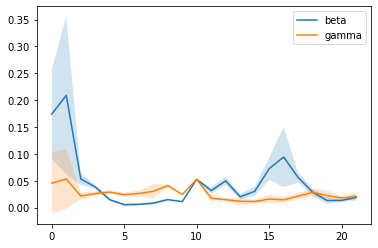
\includegraphics[width=\textwidth]{img/sir_meld_15.png}
			\caption{SIR ($10^4$ samples, $500$ resamples)}
		\end{figure}
		\column{0.4\textwidth}
		\begin{figure}
			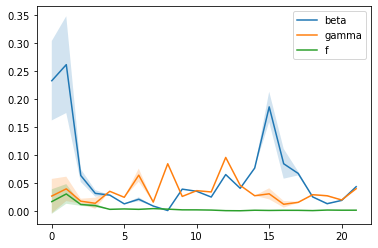
\includegraphics[width=\textwidth]{img/sird_meld_15.png}
			\caption{SIRD ($5 \cdot 10^4$ samples, $2000$ resamples)}
		\end{figure}
		\column{0.4\textwidth}
		\begin{figure}
			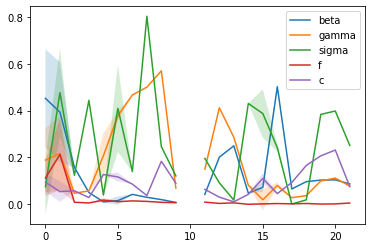
\includegraphics[width=\textwidth]{img/seird_meld_15.png}
			\caption{SEIRD ($10^5$ samples, $5000$ resamples)}
		\end{figure}
	\end{columns}
\end{frame}

\begin{frame}
	\frametitle{Bayesian melding}
	\framesubtitle{Possible sources of failure? (1/2)}
Although melding has higher potential than deterministic fitting when handling stochastic informations, its performance was worse than \texttt{curve\_fit} baseline. Possible causes of these results may be:
	\begin{itemize}
		\item observations are not really stochastic (the dataset on COVID-19 contains hard numbers and we created the pdfs synthetically),
		\item sampling was too shallow (other works on Bayesian melding applied to compartmental models suggest to use at least $10^5 \text{ -- } 10^6$ samples and $\sim 10^3$ resamples),
		\item consensus between priors and likelihoods was not reached (as evidenced by plenty of underflows during melding),
	\end{itemize}
\end{frame}

\begin{frame}
	\frametitle{Bayesian melding}
	\framesubtitle{Possible sources of failure? (2/2)}
	\begin{itemize}
		\item the model's domain and the pdfs support don't match (eg. $\beta \in [0, 1]$ for the model, but $S \in (-\infty, \infty)$ for a Gaussian pdf centered on the seed) and this adds noise during weighting (the model ``saturates'' invalid inputs, so an invalid value has the same weight as the boundary),
		\item bandwidth selection in Scipy's KDE is not optimized for multivariate case (the authors of melding propose to use Terrell's Maximum Smoothing Principle~\footfullcite{terrell1990maximal} to select automatically the best bandwidth in a scale independent and high-dimension tolerant fashion, but Scipy offers only Silverman's rule, which fails when the true distribution is very different from a Gaussian, or Scott's rule, which has similar problems~\footfullcite{silvermanscott}).
	\end{itemize}
\end{frame}

\appendix

\section{Appendix - Original project proposal slides}
\begin{frame}
	The following slides summarize some articles about Bayesian melding and were used to give an initial informal presentation about the method. They are not formatted, nor proof-read, and contain redundant content.
\end{frame}

\section{Introduction~\footfullcite{uniwa}}

\begin{frame}
	\frametitle{Bayesian melding}
	\framesubtitle{What?}
	
	Statistic technique which is used to quantify a model output's uncertainty (ie. a probability distribution over the model predictions).
	
	A deterministic model applied to a random variable produces another random variable, however posterior informations are discarded.
	
	Posterior informations may not be the direct output of the model (eg. mortality rates in COVID-19 cases are known, but a model could output the number of infected people instead).
	
\end{frame}

\begin{frame}
	\frametitle{Bayesian melding}
	\framesubtitle{Ingredients}
	
	Let's denote the inputs as $\Theta$ and a model which produces the outputs $\Phi$ as $M(\Theta) = \Phi$.
	
	We know from the real world:
	\begin{itemize}
		\item Prior on the inputs: $q(\Theta)$
		\item Data related to the outputs, which yield a posterior on the outputs $L(\Phi) = P(Data | \Phi)$
		\item Posterior on the inputs: $p(\Theta) \propto q(\Theta)L(\Phi)$ (Bayes theorem)
	\end{itemize}

	Typically we are interested not directly on the model outputs, but in quantities $\psi$ which are a function of them (with their own distributions which can give additional insight).
\end{frame}

\begin{frame}
	\frametitle{Bayesian melding}
	\framesubtitle{What can be done}
	The model can be used to estimate the output, producing another posterior on the inputs which can be different than the one achieved according to Bayes theorem.
	\begin{itemize}
		\item Better prediction: a traditional approach tends to ignore the posterior on the outputs (or to delegate it as a validation for the model), but a better approach would be to consider all the available information, similar to majority voting in an ensemble model
		\item Better coverage: traditional simulations underestimate uncertainty, taking the posteriors into account the observed values fall more often inside an interval centered at the predictions
		\item Better calibration: the output space is sampled more efficiently.
	\end{itemize}

	Typically the model is not invertible, therefore the likelihoods can be estimated only via Monte Carlo approaches.
\end{frame}

\begin{frame}
	\frametitle{Deterministic models}
	\begin{enumerate}
		\item Draw $N$ samples $\{\Theta_1, \Theta_2, \dots, \Theta_N\}$ from the prior $q(\Theta)$
		\item For each $\Theta_i$ compute the model output $\Phi_i = M(\Theta_i)$
		\item Compute weights $w_i = L(\Phi_i)$
		\item The (approximate) posterior on the inputs can be approximated by weighting $\{\Theta_1, \Theta_2, \dots, \Theta_N\}$ by $\{w_1, w_2, \dots, w_N\}$
		\item Likewise, the posterior on the quantities of interest uses the same weights on $\{\psi_1 = \Psi(\Phi_1), \psi_2 = \Psi(\Phi_2), \dots, \psi_N = \Psi(\Phi_N)\}$
	\end{enumerate}
\end{frame}

\begin{frame}
	\frametitle{Stochastic models}
	\begin{enumerate}
		\item Draw $N$ samples $\{\Theta_1, \Theta_2, \dots, \Theta_N\}$ from the prior $q(\Theta)$
		\item For each $\Theta_i$ compute the model output $J$ times obtaining $\Phi_{ij} = M(\Theta_i)$ ($j \in [1, J]$)
		\item Compute weights $w_i = L(\overline{\Phi}_i)$, where $\overline{\Phi}_i = \frac{1}{J}\displaystyle\sum_{j=1}^J \Phi_{ij}$
		\item The (approximate) posterior on the inputs can be approximated by weighting $\{\Theta_1, \Theta_2, \dots, \Theta_N\}$ by $\{w_1, w_2, \dots, w_N\}$
		\item This time, the posterior on the quantities of interest depends directly on the output distribution, without considering the weights.
	\end{enumerate}
\end{frame}



\section{Original paper~\footfullcite{poole2000inference}}
\begin{frame}
	\frametitle{Bayesian synthesis}
	Simpler method, but suffers from the Borel paradox. Given $p(\Phi, \Theta)$ (joint pre-model distribution, ie. everything known about inputs and outputs from the real world, except what is modeled deterministically) and the model $M: \Theta \mapsto \Phi$, the post-model distribution is:
	\begin{equation*}
		\begin{cases}
		p(\Theta, M(\Theta))&if\ \Phi = M(\Theta)\\
		0&otherwise
		\end{cases}
	\end{equation*}
	
	Applying the Bayes theorem, $p(\Theta, \Phi) \propto q_1(\Theta) q_2(\Phi) L_1(\Theta) L_2(\Phi)$, where the distribution has been decomposed in terms of priors (q) and likelihoods (L) on inputs and outputs.
	
	Sample importance resampling is used to get a prediction.
\end{frame}

\begin{frame}
	\frametitle{Borel paradox}
	The way the post-model distribution is defined in Bayesian synthesis is ill posed and its values depend on how the model is parametrized (a counter-example was given by simply modeling an exponential growth model and computing input distributions in linear or log scale and observing different results).
	
	More generally, the Borel paradox manifests itself if a conditional distribution is defined on an event with probability 0.
	
	The paradox in Bayesian synthesis is not due to likelihoods ($L_1$ and $L_2$, which are invariant wrt reparametrization), but due to prior distributions. Intuitively this is caused by the fact that from the input prior $q_1(\Theta)$ and the model $M(\Theta)$ another prior on the outputs ($q_1^*(\Phi)$) can be derived and may be different from $q_2(\Phi)$.
\end{frame}

\begin{frame}
	\frametitle{Bayesian melding as consensus pooling}
	Assuming a ``coherent'' prior $\tilde{q}$ can be derived, applying Bayes theorem yields $\tilde{q}(\Theta)L_1(\Theta)L_2(M(\Theta))$ which is a traditional Bayes posterior and only marginal distributions (instead of pre-model and post-model distributions) are needed.
	
	Sample importance resampling is still required due to the impossibility of deriving the inverse of the model analytically.
	
	Finding $\tilde{q}$ can be seen as determining the consensus in an ensemble. Pooling different distributions is a statistical way of determining consensus.
	
	External Bayesianity is the property of a pooling method which guarantees posterior invariance with respect to forming the multivariate prior and then applying Bayes theorem or, viceversa, applying Bayes theorem on the univariate priors and then forming the multivariate posterior.
\end{frame}

\begin{frame}
	\frametitle{Logarithmic pooling}
	\begin{equation*}
		T(q_1, q_2, \dots, q_n) \propto \displaystyle\prod_{i=1}^n q_i^{\alpha_i},\ with\ \displaystyle\sum_{i=1}^n \alpha_i = 1
	\end{equation*}
	Logarithmic pooling is the only mechanism which satisfies external Bayesianity, it's also invariant wrt rescaling of priors and naturally sets to zero the pooled distribution if one of the priors is zero for a given value (zero preservation property, important in melding because allows to easily eliminate ``impossible'' values according to model or evidences).
	
	For two distributions (the model output and the evidence), only $\alpha$ and $1 - \alpha$ are used and the value of $\alpha$ is arbitrary and tunes ``reliability'' of the distributions (not precision of melding). Geometric pooling is logarithmic pooling with $\alpha = \frac{1}{2}$ (ie. same importance to model and evidence).
\end{frame}

\begin{frame}
	\frametitle{Sample importance resampling algorithm}
	On a non-invertible model pooling still produces unambiguous results, however inference on the inputs does not. SIR works both for continuous and discrete models, even when they are non-invertible or hard to compute.
	
	\begin{enumerate}
		\item Draw $k$ samples of $\Theta$ from the prior $q_1(\Theta)$
		\item For each $\Theta_i$ run the model to get $\Phi_i$
		\item Estimate $q_i^*(\Phi)$ with nonparametric density estimation (eg. KDE with Gaussian kernel)
		\item Create weights $w_i = (\frac{q_2(M(\Theta_i))}{q_1^*(M(\Theta_i))})^{1-\alpha} L_1(\Theta_i) L_2(M(\Theta_i))$
		\item Sample $l$ values with probabilities proportional to $w_i$, which will be an approximation of the posterior.
	\end{enumerate}

	SIR may be slow with complex models and large numbers of samples. Improved algorithms are available in literature.
	
\end{frame}

\begin{frame}
	\frametitle{Model validation}
	``Goodness'' can be defined as the property of a model to produce for any input, output or quantity of interest, a ``substantial overlap'' with the other sources of informations (priors on inputs, priors on outputs, likelihoods on inputs and likelihoods on outputs, where some of them may be unavailable).
	
	Given two distributions, the overlap can be estimated qualitatively by sampling random values and observing the boxplots (which should be more or less of the same size and around the same mean).
	
	\begin{itemize}
		\item Prior on the outputs: $q_2(\Phi)$ is compared with $q_2^*(\Phi)$ (which is induced by the prior on the inputs)
		\item Prior on the inputs: $q_1^*(\Theta)$ is computed as the pooled prior with $\alpha = 0$ (ie. pooling considering only the model) and then compared with $q_1(\Theta)$
		\item Likelihoods need an heuristic to determine $L_1^*(\Theta)$ and $L_2^*(\Phi)$ distributions comparable with their counterparts.
	\end{itemize}
	
\end{frame}

\begin{frame}
	\frametitle{Hypothesis testing}
	Given two models $M_0$ (null) and $M_1$ (alternative), a Bayes factor $B_{10}$ can be computed and if it's less than 1, the null model explains better the evidence, while above the alternative is better:
	\begin{itemize}
		\item Between 1 and 3 the evidence on the alternative being better is weak
		\item Between 3 and 20 the evidence on the alternative being better is positive
		\item Between 20 and 100 the evidence on the alternative being better is strong
		\item Above 100 the evidence on the alternative being better is very strong.
	\end{itemize}

	The Bayesian factor can be computed by modifying slightly the SIR implementation for Bayesian melding.
\end{frame}

\begin{frame}
	\frametitle{Relabeling}
	In some cases the model may be reformulated by relabeling some inputs as outputs (or viceversa), eg. instead of knowing the values at time $0$ and regressing at time $t$, it may be desirable to regress time $0$ knowing the values at $t$.
	
	If the variants of the model $M$ are $\tau = M_1(\lambda, \gamma)$ and $\lambda = M_2(\tau, \gamma)$ (where $\gamma$ are the shared inputs and the other two are variables which form the input for one model but the output of the other one) and the transformation $(\lambda, \gamma) \mapsto (\tau, \gamma)$ is one-to-one, then Bayesian melding can be applied on the (independent) priors $q_1(\lambda)$, $q_2(\gamma)$ and $q_3(\tau)$ (taking care on how pooling is done to consistently determine weights for both variants).
\end{frame}

\section{Melding on deterministic models~\footfullcite{alkema2008bayesian}}
\begin{frame}
	\frametitle{Melding on time series}
	Plausibility bounds for HIV prevalence were given by experts, but lacked a formal statistical assessment (ie. they were not confidence intervals).
	
	Bayesian melding was used to calibrate the prediction curves of an EPP model (deterministic).
	
	Sampling prevalence curves: from the posterior on HIV prevalence SIR (sampling importance resample) algorithm was used:
	\begin{enumerate}
		\item Sample a large number of input parameters (according to their prior joint distribution)
		\item Run the model to obtain a time series for each input
		\item Compute weights based on how well the prediction fits the actual data (ie. $w_i = p(M(\Theta_i)|\Phi)$)
		\item Resample input parameters with a probability proportional to weights and rerun the model
	\end{enumerate}

	The input samples should be large enough (eg. 200000) to cover the input space and to produce a reasonable number of unique predictions. Resampling can be done with a much lower number of runs (eg. 3000).
	
\end{frame}

\begin{frame}
	\frametitle{Curve calibration based on known posterior}
	ANCs (antenatal curves) are used to estimate HIV prevalence, however these data differ from population prevalence. Population-based surveys are used to meld the ANC curves and get a better estimate.
	
	\begin{enumerate}
		\item Rescale the time series based on the surveys (eg. shift by the mean and multiply by the variance)
		\item Compute weights (based on the surveys' data, NOT the ANC curves)
		\item Resample
	\end{enumerate}
\end{frame}

\begin{frame}
	\frametitle{Curve calibration based on similar data}
	ANCs (antenatal curves) are used to estimate HIV prevalence, however these data differ from population prevalence.
	If population-based surveys are unavailable, melding is performed against different countries which have those data.
	
	Assume that the difference between ANC and surveys is given by a bias (which is unknown since surveys are missing in this case), the mean and variance of which can be estimated by data on other countries.
	
	\begin{enumerate}
		\item Compute mean and variance of bias (difference between ANC and survey data) in other countries
		\item Rescale the time series based on the bias
		\item Resample
	\end{enumerate}
\end{frame}

\begin{frame}
	\frametitle{Best trajectory}
	The best trajectory is given by the most likely prediction given prior and data (maximum a posteriori trajectory, MAP).
	
	Due to Bayes theorem, the posterior probability is given by the product of prior on input, prior on output and likelihood of data.
	
	The model is run for subpopulations (eg. rural vs urban areas), the posteriors are weighted by population size and the MAP is selected for the national trajectory. Confidence intervals can be evaluated on the MAP.

\end{frame}


\section{Weights for little data~\footfullcite{hotta2010bayesian}}

\begin{frame}
	\frametitle{Best trajectory using limited data}
	Sample importance resampling algorithm was applied to a SEIR model on co-infection of HIV and tuberculosis on prison inmates (the removal rate included deaths, recoveries and releases from prison), with a lot of missing data (eg. if the inmates had HIV before entering prison). A priori distributions of HIV and TB cases are assumed independent.
	
	The simulations were too few to get a good estimate of weights for resampling, so they were approximated by a multivariate normal, using means and variances from the posterior (symptomatic cases).
	
	This procedure still achieved better results than least square error estimation on a Monte Carlo Markov Chain simulation on the same model applied to the same priors.
	
\end{frame}

\section{Exploit posterior knowledge to improve deterministic models~\footfullcite{sanchez2020many}}
\begin{frame}
	\frametitle{SEIR model}
	\begin{itemize}
		\item 95 age groups for age-specific morality rates
		\item Isolation explicitly modeled
		\item Infectious period after testing
		\item $E$ and $I$ (one for each age group) components are split into $E^u$, $E^d$, $I^u$ and $I^d$ (undetected and detected fractions)
		\item $E^d$ is assumed to be quarantined
		\item $R$ (recoveries) and $D$ deaths are modeled separately
		\item $M$ (death by other causes) and $M^c(\varepsilon)$ (death by COVID-19) diagonal matrix of death rates for each of the 95 age groups. $\varepsilon$ is the symptomatic fraction (the lower it is, the higher the divergence between the true fatality rate and the estimated one)
		\item Time steps are daily.
	\end{itemize}
	
\end{frame}

\begin{frame}
	\frametitle{Calibration}
	Deaths are more reliable than the positive tests, even when the country decides to count as COVID-19 deaths only those of people who were tested positive.
	
	Ordinary least square regression to model the age gradient in mortality (in log scale), very good fit after 30 years of age.
	
	Prior on $\varepsilon$ was set to be uniform in $]0; 1[$ and the mortality matrices were built by adjusting from annual to daily rates and by unpacking age groups with a penalized composite link model (the official statistics in the human mortality database are grouped in 5-years bins) and smoothed with a Kannisto model after 80 years of age.
\end{frame}

\begin{frame}
	\frametitle{Priors}
	Epidemiological characteristics of COVID-19 are still unknown, so all priors are uninformative (ie. uniform distributions between a minimum and a maximum value for each variable $S, E^u, E^d, I^u, I^d, R, D$).
	
	Parameters are taken from the literature, except for $\varepsilon$ which is sampled between 0 and 1.
	
	Time $s$ of the SEIR model is the number of days elapsed from the first death by COVID-19 in the country. An additional variable $T$ models the time instant in which quarantine measures start to slow down spreading. Before $T$ deaths reported can have an high error, so the joint prior on the outputs is uninformative as well (1 if the error at time $T$ is less than the maximum error up to time $T$, 0 otherwise).
\end{frame}

\begin{frame}
	\frametitle{Melding}
	Weights were computed with geometric pooling on the priors $q_1^\alpha \cdot q_2^{1-\alpha}$ ($q_1$ prior on the inputs, $q_2$ prior on the outputs, $\alpha = 0.5$ to give the same importance to model and data).
	
	Posteriors on the input were estimated using a standard gaussian KDE.
\end{frame}

\end{document}